%! TEX root = main.tex

\begin{frame}\frametitle{\insertsubsection}
Let us recall the Eratosthenes sieving method:
\begin{figure}\centering
  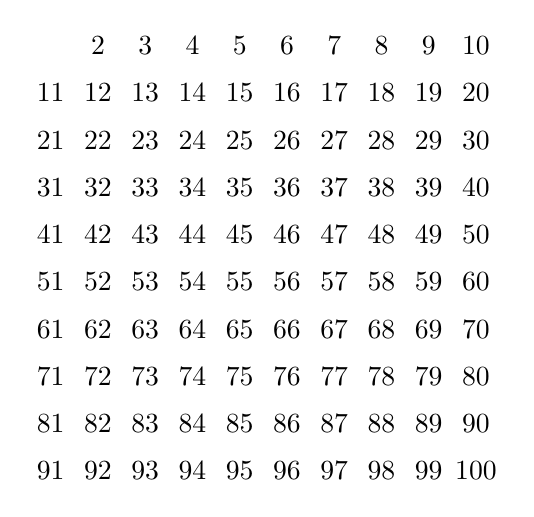
\begin{tikzpicture}[scale=0.6]
    \foreach \i in {0,...,9} \foreach \j in {0,...,9} {
      \pgfmathtruncatemacro{\result}{\i * 10 + \j + 1}
      \ifnum\result>1
        \node at (\j, -\i) {\result};
      \fi
    }
  \end{tikzpicture}
\end{figure}
\end{frame}

\begin{frame}\frametitle{\insertsubsection}
Let us recall the Eratosthenes sieving method:
\begin{figure}\centering
  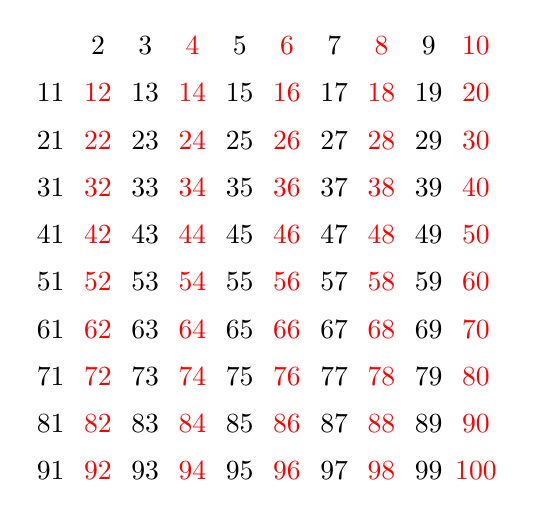
\begin{tikzpicture}[scale=0.6]
    \foreach \i in {0,...,9} \foreach \j in {0,...,9} {
      \pgfmathtruncatemacro{\result}{\i * 10 + \j + 1}
      \ifnum\result>1 {
        \def\mycolor{black}
        \pgfmathparse{int(mod(\result,2))}
        \ifnum\pgfmathresult=0\ifnum\result>2\def\mycolor{red}\fi\fi
        \node[text=\mycolor] at (\j, -\i) {\result};
      } \fi
    }
  \end{tikzpicture}
\end{figure}
\end{frame}

\begin{frame}\frametitle{\insertsubsection}
Let us recall the Eratosthenes sieving method:
\begin{figure}\centering
  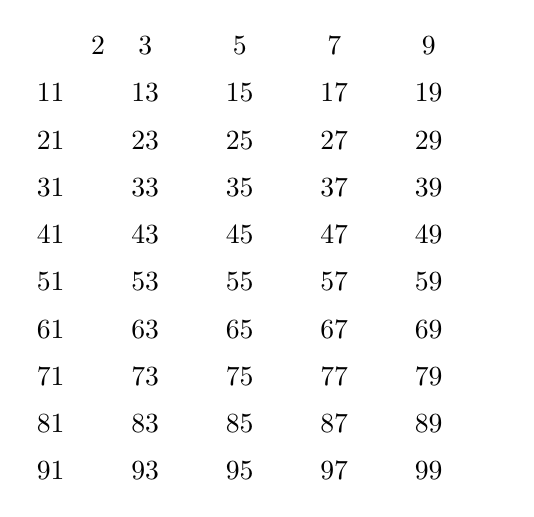
\begin{tikzpicture}[scale=0.6]
    \foreach \i in {0,...,9} \foreach \j in {0,...,9} {
      \pgfmathtruncatemacro{\result}{\i * 10 + \j + 1}
      \ifnum\result>1 {
        \pgfmathparse{int(mod(\result,2))}
        \def\mycolor{black}
        \ifnum\pgfmathresult=0\ifnum\result>2\def\mycolor{white}\fi\fi
        \node[text=\mycolor] at (\j, -\i) {\result};
      } \fi
    }
  \end{tikzpicture}
\end{figure}
\end{frame}

\begin{frame}\frametitle{\insertsubsection}
Let us recall the Eratosthenes sieving method:
\begin{figure}\centering
  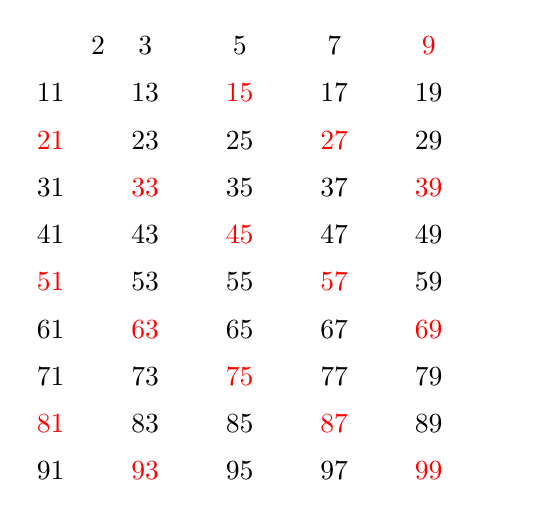
\begin{tikzpicture}[scale=0.6]
    \foreach \i in {0,...,9} \foreach \j in {0,...,9} {
      \pgfmathtruncatemacro{\result}{\i * 10 + \j + 1}
      \ifnum\result>1 {
        \def\mycolor{black}
        \pgfmathparse{int(mod(\result,3))}
        \ifnum\pgfmathresult=0\ifnum\result>3\def\mycolor{red}\fi\fi
        \pgfmathparse{int(mod(\result,2))}
        \ifnum\pgfmathresult=0\ifnum\result>2\def\mycolor{white}\fi\fi
        \node[text=\mycolor] at (\j, -\i) {\result};
      } \fi
    }
  \end{tikzpicture}
\end{figure}
\end{frame}

\begin{frame}\frametitle{\insertsubsection}
Let us recall the Eratosthenes sieving method:
\begin{figure}\centering
  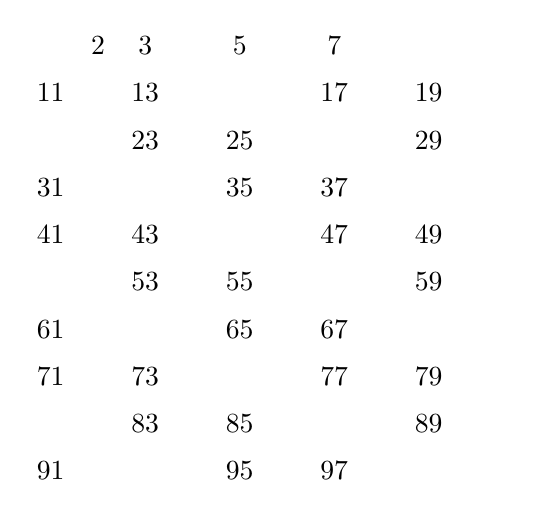
\begin{tikzpicture}[scale=0.6]
    \foreach \i in {0,...,9} \foreach \j in {0,...,9} {
      \pgfmathtruncatemacro{\result}{\i * 10 + \j + 1}
      \ifnum\result>1 {
        \def\mycolor{black}
        \pgfmathparse{int(mod(\result,2))}
        \ifnum\pgfmathresult=0\ifnum\result>2\def\mycolor{white}\fi\fi
        \pgfmathparse{int(mod(\result,3))}
        \ifnum\pgfmathresult=0\ifnum\result>3\def\mycolor{white}\fi\fi
        \node[text=\mycolor] at (\j, -\i) {\result};
      } \fi
    }
  \end{tikzpicture}
\end{figure}
\end{frame}

\begin{frame}\frametitle{\insertsubsection}
Let us recall the Eratosthenes sieving method:
\begin{figure}\centering
  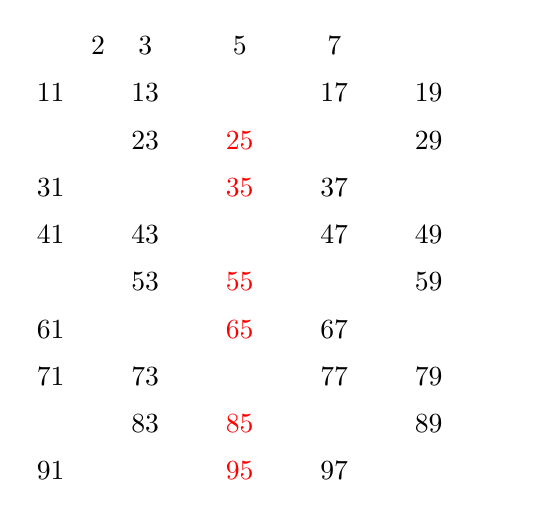
\begin{tikzpicture}[scale=0.6]
    \foreach \i in {0,...,9} \foreach \j in {0,...,9} {
      \pgfmathtruncatemacro{\result}{\i * 10 + \j + 1}
      \ifnum\result>1 {
        \def\mycolor{black}
        \pgfmathparse{int(mod(\result,5))}
        \ifnum\pgfmathresult=0\ifnum\result>5\def\mycolor{red}\fi\fi
        \pgfmathparse{int(mod(\result,2))}
        \ifnum\pgfmathresult=0\ifnum\result>2\def\mycolor{white}\fi\fi
        \pgfmathparse{int(mod(\result,3))}
        \ifnum\pgfmathresult=0\ifnum\result>3\def\mycolor{white}\fi\fi
        \node[text=\mycolor] at (\j, -\i) {\result};
      } \fi
    }
  \end{tikzpicture}
\end{figure}
\end{frame}

\begin{frame}\frametitle{\insertsubsection}
Let us recall the Eratosthenes sieving method:
\begin{figure}\centering
  \begin{tikzpicture}[scale=0.6]
    \foreach \i in {0,...,9} \foreach \j in {0,...,9} {
      \pgfmathtruncatemacro{\result}{\i * 10 + \j + 1}
      \ifnum\result>1 {
        \def\mycolor{black}
        \pgfmathparse{int(mod(\result,2))}
        \ifnum\pgfmathresult=0\ifnum\result>2\def\mycolor{white}\fi\fi
        \pgfmathparse{int(mod(\result,3))}
        \ifnum\pgfmathresult=0\ifnum\result>3\def\mycolor{white}\fi\fi
        \pgfmathparse{int(mod(\result,5))}
        \ifnum\pgfmathresult=0\ifnum\result>5\def\mycolor{white}\fi\fi
        \node[text=\mycolor] at (\j, -\i) {\result};
      } \fi
    }
  \end{tikzpicture}
\end{figure}
\end{frame}

\begin{frame}\frametitle{\insertsubsection}
Let us recall the Eratosthenes sieving method:
\begin{figure}\centering
  \begin{tikzpicture}[scale=0.6]
    \foreach \i in {0,...,9} \foreach \j in {0,...,9} {
      \pgfmathtruncatemacro{\result}{\i * 10 + \j + 1}
      \ifnum\result>1 {
        \def\mycolor{black}
        \pgfmathparse{int(mod(\result,7))}
        \ifnum\pgfmathresult=0\ifnum\result>7\def\mycolor{red}\fi\fi
        \pgfmathparse{int(mod(\result,2))}
        \ifnum\pgfmathresult=0\ifnum\result>2\def\mycolor{white}\fi\fi
        \pgfmathparse{int(mod(\result,3))}
        \ifnum\pgfmathresult=0\ifnum\result>3\def\mycolor{white}\fi\fi
        \pgfmathparse{int(mod(\result,5))}
        \ifnum\pgfmathresult=0\ifnum\result>5\def\mycolor{white}\fi\fi
        \node[text=\mycolor] at (\j, -\i) {\result};
      } \fi
    }
  \end{tikzpicture}
\end{figure}
\end{frame}

\begin{frame}\frametitle{\insertsubsection}
Let us recall the Eratosthenes sieving method:
\begin{figure}\centering
  \begin{tikzpicture}[scale=0.6]
    \foreach \i in {0,...,9} \foreach \j in {0,...,9} {
      \pgfmathtruncatemacro{\result}{\i * 10 + \j + 1}
      \ifnum\result>1 {
        \def\mycolor{black}
        \pgfmathparse{int(mod(\result,2))}
        \ifnum\pgfmathresult=0\ifnum\result>2\def\mycolor{white}\fi\fi
        \pgfmathparse{int(mod(\result,3))}
        \ifnum\pgfmathresult=0\ifnum\result>3\def\mycolor{white}\fi\fi
        \pgfmathparse{int(mod(\result,5))}
        \ifnum\pgfmathresult=0\ifnum\result>5\def\mycolor{white}\fi\fi
        \pgfmathparse{int(mod(\result,7))}
        \ifnum\pgfmathresult=0\ifnum\result>7\def\mycolor{white}\fi\fi
        \node[text=\mycolor] at (\j, -\i) {\result};
      } \fi
    }
  \end{tikzpicture}
\end{figure}
\pause
We can stop here, as the next remaining number is \(11\), and \(11^2 > 100\).
\end{frame}

\begin{frame}\frametitle{Eratosthenes Sieve}
Tada! We obtained the primes below \(100\):
\[
  2, 3, 5, 7, 11, 13, 17, 19, 23, 29, 31, 37, 41, 43
\]
\[
  47, 53, 59, 61, 67, 71, 73, 79, 83, 89, 97
\]
\end{frame}
